\chapter{Transformations}
\section{Coordinates}
When trying to understand transformations it is a good idea to start off by looking at the coordinate system and that is what we will do here.  The system that we will use here describes the position of a point by saying how far it is across from an origin and how far up it is from an origin in that order.  We usually show this information as a pair of numbers in brackets seperated by a comma.

e.g. (5, 7)

which means 5 to the right and 7 up from the origin
\begin{center}
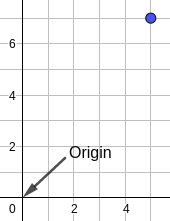
\includegraphics[scale=0.5]{./Images/Transformations/Basic_Coords.png}
\end{center}
We call the first number in the coordinate pair the $x$ coordinate and the second number the $y$ coordinate.

\begin{exmp}
Let's look at the diagram below and give the coordinates of the points.
\begin{center}
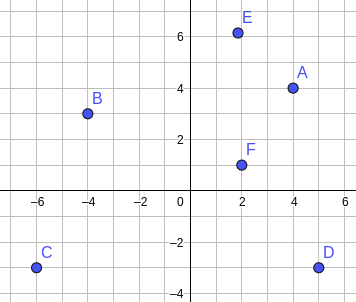
\includegraphics[scale=0.5]{./Images/Transformations/Coord_eg_1.png}
\end{center}
All the coordinates are done relative to the origin.

We can see that 'A' is 4 to the right and 4 up, so it's coordinates are $(4, 4)$

We can see that 'B' is 4 to the left and 3 up, so it's coordinates are $(-4, 3)$

We can see that 'C' is 6 to the left and 3 down, so it's coordinates are $(-6, -3)$

We can see that 'D' is 5 to the right and 3 down, so it's coordinates are $(5, -3)$

We can see that 'E' is 2 to the right and 6 up, so it's coordinates are $(2, 6)$

We can see that 'F' is 1 to the right and 1 up, so it's coordinates are $(2, 1)$
\end{exmp}
\subsection{Exercise}
Find the coordinates of the following points
\begin{center}
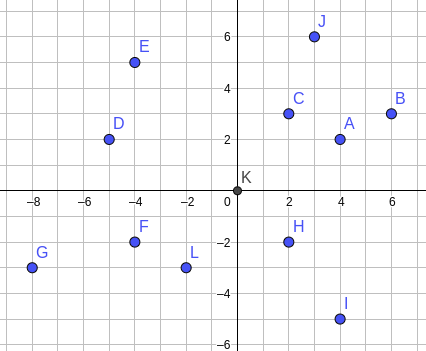
\includegraphics[scale=0.5]{./Images/Transformations/Coords_Ex_1.png}
\end{center}

\begin{exmp}
	Plot the following coordinates one after the other and joining them with a line:

	$(0, 0)$, $(2, 2)$, $(4, 2)$, $(7, 0)$, $(4, -2)$, $(2, -2)$ and $(0,0)$

	Now on the same grid do the same with these points

	$(2, 0)$, $(3, 1)$, $(4, 0)$ and $(3, -1)$

	We should end up with a really bad picture of an eye
	\begin{center}
	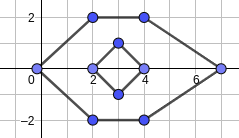
\includegraphics[scale=0.5]{./Images/Transformations/Coord_eg_2.png}
	\end{center}
\end{exmp}

\subsection{Exercise}
Design your own picture with a set of instructions so that a friend can try and recreate your design.
\section{Translations}
A translation is when we move an object so that its position has changed, but nothing else, it will still be the same size and will not have been rotated.

We will describe our translations by saying how far the shape has moved to the right and how far it has moved up.

\begin{exmp}
	Consider the shape ABC below and the translated shape A'B'C'
	\begin{center}
	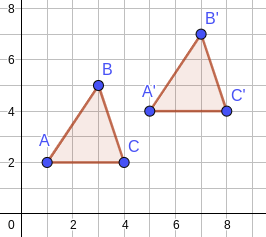
\includegraphics[scale=0.5]{./Images/Transformations/Trans_eg_1.png}
	\end{center}
	Every point has been translated 4 right and 2 up
\end{exmp}

\begin{exmp}
	Consider the shape ABC below and the translated shape A'B'C'
	\begin{center}
	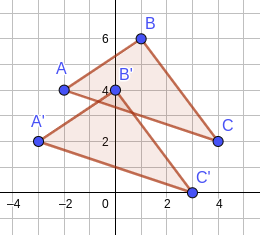
\includegraphics[scale=0.5]{./Images/Transformations/Trans_eg_2.png}
	\end{center}

	Every point has been translated 1 left and 2 down
\end{exmp}

\begin{exmp}
	You can also translate a point
	\begin{center}
	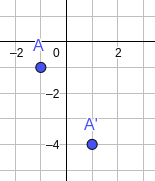
\includegraphics[scale=0.5]{./Images/Transformations/Trans_eg_3.png}
	\end{center}

	The point has been translated 2 right and 3 down
\end{exmp}

\subsection{Exercise}
Describe each of the translations below.  The first one is done for you:

	\begin{center}
		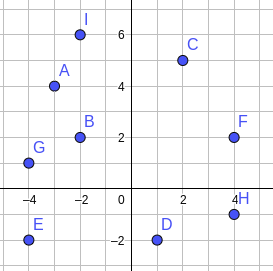
\includegraphics[scale=0.6]{./Images/Transformations/Trans_ex_1.png}
	\end{center}

	\begin{enumerate}
		\item $A \rightarrow B$ right 1, down 2
		\item $A \rightarrow C$ ...
		\item $H \rightarrow D$ ...
		\item $D \rightarrow H$ ...
		\item $E \rightarrow I$ ...
		\item $H \rightarrow E$ ...
		\item $H \rightarrow A$ ...
		\item $B \rightarrow I$ ...
		\item $F \rightarrow F$ ...
		\item $G \rightarrow E$ ...
		\item $D \rightarrow C$ ...
		\item $C \rightarrow G$ ...
	\end{enumerate}

\subsection{Exercise}
	If we had a general point $(x,y)$ and we described its translation as $(x,y) \rightarrow (x+2,y-4)$

	This would mean the translation was 2 right, 4 down.

	Describe the following translations:
	\begin{enumerate}
		\item $(x,y) \rightarrow (x+3,y+5)$
		\item $(x,y) \rightarrow (x-6,y+1)$
		\item $(x,y) \rightarrow (x,y-4)$
		\item $(x,y) \rightarrow (x+4,y)$
	\end{enumerate}

	We can also display a translation with a vector where we show the hoizontal move above the vertical move.
\section{Reflections}
When we are reflecting a shape in here we will be doing it on a coordinate axis.  The easiest way to do this, is to just reflect the points and join them together with the corresponding lines.  Consider the diagram below where we reflect our shape in the y-axis.

\bigskip

	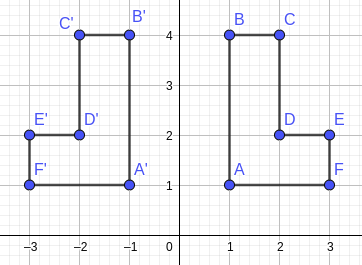
\includegraphics[scale=0.6]{./Images/Transformations/Reflections_ex_1.png}

\bigskip

The shape has been reflected in the y-axis.  To find the position of a reflected point we simple move the point directly to the line, covering the shortest distance, and then carryon the same distance again on the other side.  In our example we can see that (A) moved 1 square and 1 square and that (D) moved 2 squares and 2 squares.

\bigskip

	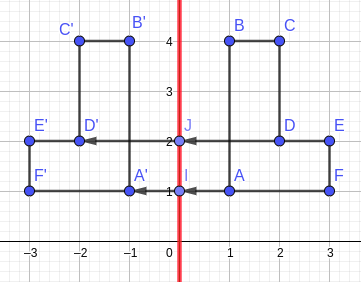
\includegraphics[scale=0.6]{./Images/Transformations/Reflections_ex_2.png}

\bigskip

\begin{exmp}
	Reflect the point $(4,7)$ in the y-axis and the point $(3, -2)$ in the x-axis.
	First we plot the points.

	\bigskip

		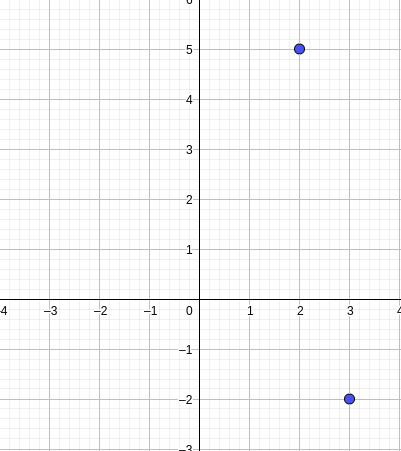
\includegraphics[scale=0.6]{./Images/Transformations/Reflections_ex_3.png}

	\bigskip

	Then we reflect the points in their respective lines

	\bigskip

		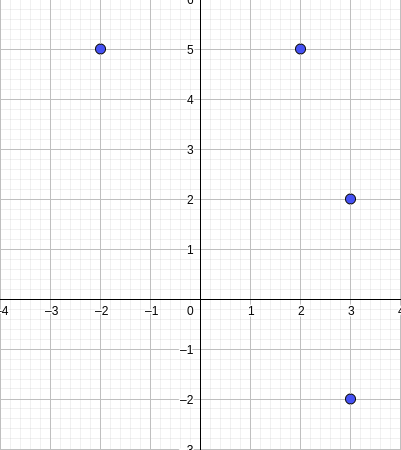
\includegraphics[scale=0.6]{./Images/Transformations/Reflections_ex_4.png}

	\bigskip

	So $(4,7) \rightarrow (-4,7)$ and $(3, -2) \rightarrow (3, 2)$
\end{exmp}
\subsubsection{Exercise}
Reflect each of the points below in the y-axis
	\begin{enumerate}
		\item $(3, 8)$
		\item $(4, -5)$
		\item $(-6, 5)$
		\item $(-2, -7)$
		\item $(3, 2)$
		\item $(7, 1)$
		\item $(3, -3)$
		\item $(0, 5)$
		\item $(0, 5)$
	\end{enumerate}
	Reflect the points below in the x-axis
	\begin{enumerate}
		\item $(3, 8)$
		\item $(4, -5)$
		\item $(-6, 5)$
		\item $(-2, -7)$
		\item $(3, 2)$
		\item $(7, 1)$
		\item $(3, -3)$
		\item $(0, 5)$
		\item $(5, 0)$
	\end{enumerate}

\subsection{Exercise}
	Verify that if we reflect the point $(3, 2)$ in the vertical line $x = 2$ we get the point $(1, 2)$
	\bigskip

		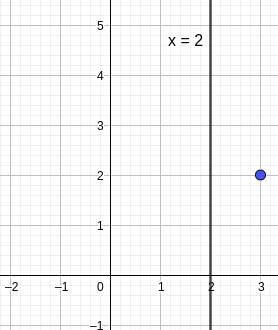
\includegraphics[scale=0.6]{./Images/Transformations/Reflections_ex_5.png}

	\bigskip

	Reflect each of the points below in the line $x = 1$
		\begin{enumerate}
			\item $(3, 8)$
			\item $(4, -5)$
			\item $(-6, 5)$
			\item $(-2, -7)$
			\item $(3, 2)$
			\item $(7, 1)$
			\item $(3, -3)$
			\item $(0, 5)$
		\end{enumerate}
		Reflect each of the points below in the line $y=-2$
			\begin{enumerate}
				\item $(3, 8)$
				\item $(4, -5)$1
				\item $(-6, 5)$
				\item $(-2, -7)$
				\item $(3, 2)$
				\item $(7, 1)$
				\item $(3, -3)$
				\item $(0, 5)$
				\item $(0, 5)$
			\end{enumerate}
	\subsection{Algebraic Mapping}
	We looked at the idea of describing a translation algebraically in the last section.  We can do the same for translations.  Hopefully you noticed that when we reflected a point in the y-axis that the y value stayed the same and that the x value changed sign.  The mapping to represent this is $(x, y) \rightarrow (-x, y)$.

	\bigskip

	What is the mapping for a reflection in the x-axis?

	\begin{exmp}
		What is the mapping for a reflection in the line $x = 2$?

	\bigskip

		We know that the y value does not change.  We also know how to reflect in the y-axis, so the first thing we need to do is move everything 2 to the left so we get the mapping:

	\bigskip

		$(x,y) \rightarrow (x-2, y)$

	\bigskip

		Now we can reflect this in the y-axis to get:

	\bigskip

		$(x-2,y) \rightarrow (-x+2, y)$

	\bigskip

		Now we have to move it back, 2 to the right, to get:

		$(x, y) \rightarrow (-x + 4, y)$
	\end{exmp}

\subsection{Exercise}
Find the mappings for the following reflections:
\begin{enumerate}
	\item In the line $x=1$
	\item In the line $x=4$
	\item In the line $x=-2$
	\item In the line $y=2$
	\item In the line $y=-3$
	\item In the line $y=1$
\end{enumerate}

\subsection{Rotations}
We will only consider rotations about the origin in multiples of $90^o$ (clockwise and Anti-clockwise).

\subsubsection{Rotate a point on an axis}
The diagram below shows the point $(0, 3)$ being rotated $90^o$ clockwise about the origin.

\bigskip

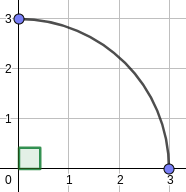
\includegraphics[scale=0.6]{./Images/Transformations/Rotations_axis.png}

\bigskip

The simple case is to rotate a point about on an axis.  You can see from the diagram that when we rotate a point it just moves to another axis, the same distance from the origin.  So when we rotate $90^o$ about the origin the point $(0, 4)$ goes to the point $(4,0)$ and that the point $(-2, 0)$ goes to $(0, 2)$

\subsubsection{Exercise}
Rotate each of the points below to give the required coordinates
\begin{enumerate}
    \item $(0, 3)$ clockwise $90^o$
    \item $(4, 0)$ anticlockwise $90^o$
    \item $(-2, 0)$ clockwise $90^o$
    \item $(0, -5)$ clockwise $90^o$
    \item $(0, 7)$ clockwise $180^o$
    \item $(0, 7)$ anticlockwise $180^o$
    \item $(1, 0)$ clockwise $90^o$
    \item $(0, -1)$ clockwise $90^o$
    \item $(-1, 0)$ clockwise $90^o$
    \item $(0, 1)$ clockwise $90^o$
\end{enumerate}

\subsection{Rotate any point about the origin}
The best way to do this is to imagine that the axes are rotating and place the point in its new place accordingly.
Consider the picture below:

\bigskip

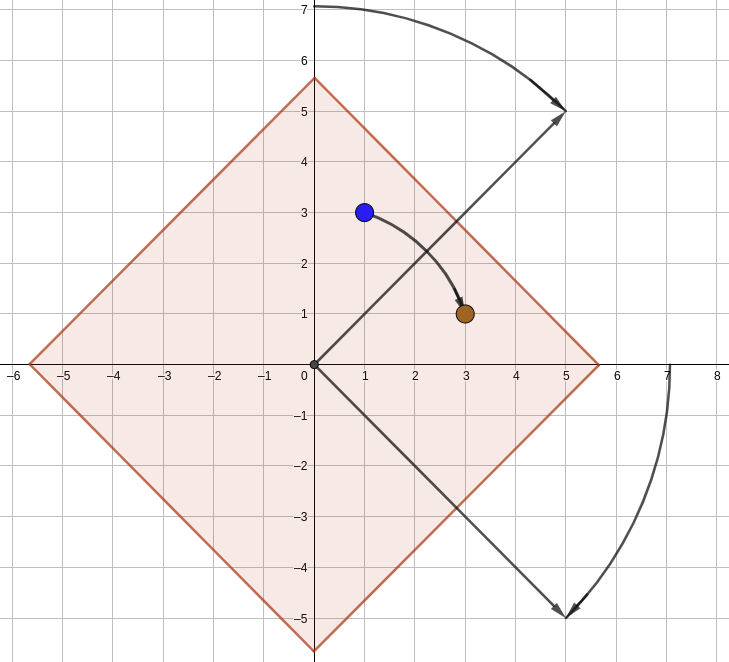
\includegraphics[scale=0.4]{./Images/Transformations/Rotation_1.png}

\bigskip

In this picture the rotation is $45^o$ clockwise about the origin.  You can see the point before the rotation is 1 across and 3 up.  Now the axes have rotated and the point is still 1 across and 3 up with respect to the new axes which puts it in the actual position of 3 across and 1 up.  If we had rotated by $90^o$ the point would be at the position 3 across and 1 down.

\subsubsection{Exercise}
For all the points below rotate them clockwise $90^o$ about the origin.
\begin{enumerate}
	\item $(3, 5)$
	\item $(5, 3)$
	\item $(1, 1)$
	\item $(2, 4)$
	\item $(7, 3)$
	\item $(6, 5)$
	\item $(2, 2)$
	\item $(1, 5)$
	\item $(3, 7)$
	\item $(9, 5)$
	\item Describe how to work out what happens when a point in this area is rotated clockwise $90^o$ about the origin.
\end{enumerate}

\subsubsection{Exercise}
For all the points below rotate them clockwise $90^o$ about the origin.
\begin{enumerate}
	\item $(-3, 5)$
	\item $(5, -3)$
	\item $(1, -1)$
	\item $(-2, 4)$
	\item $(-7, 3)$
	\item $(6, -5)$
	\item $(2, -2)$
	\item $(-1, 5)$
	\item $(-3, -7)$
	\item $(-9, -5)$
	\item Describe how to work out what happens when a point is rotated clockwise $90^o$ about the origin.
\end{enumerate}
\section{Combinations}
In this section we will see what happens when we do one transformation after another.
\subsubsection{Exercise}
Verify the transformations below.
\begin{enumerate}
	\item $(2, 5)$ is translated 2 right and 3 down then reflected in the y-axis, its new position is $(-4, 2)$
	\item $(-2, -3)$ is reflected in the x-axis and then rotated $90^o$ clockwise about the origin, its new position is $(3, 2)$
	\item $(3, -1)$ is reflected in the x-axis and then reflected in the y-axis, its new position is $(-3, 1)$
	\item $(3, -1)$ is reflected in the y-axis and then reflected in the x-axis, its new position is $(-3, 1)$
\end{enumerate}
